\newgeometry{right=30mm, left=15mm, top=20mm, bottom=20mm,}
\lhead{Name:}
\section*{Topic Test:}
\subsection*{MA-T1 Trigonometry and Measure of Angles}
\subsection*{MA-T2 Trigonometric Functions and Identities}

\vpword{Marks}
%\multicolumngradetable{3}[questions]

\begin{questions}
\question[1]
    Find the value of $\theta$ such that $\cos ( \theta + 25^{\circ}) = \sin (10^{\circ} + \theta) $.
    \fillwithdottedlines{25mm}

    \question Find the exact value of:
    \begin{parts}
        \part[1] $\tan \dfrac{7 \pi}{4}$.
        \fillwithdottedlines{17mm}
        \part[1] $\cos 930^{\circ}$
        \fillwithdottedlines{17mm}
    \end{parts}

\question
    It is known that $\tan \alpha = 1.4$, where $0^{\circ} < \alpha < 90^{\circ}$.
    \begin{parts}
        \part[2] Find the exact value of $\mathrm{cosec}^{2} \alpha$.
        \fillwithdottedlines{25mm}
        \part[2] Find the exact value of $ \cos \left(270^{\circ} - \alpha \right)$.
        \fillwithdottedlines{25mm}
    \end{parts}

\newpage

\question
    A stunt pilot flies at an average speed of 30 m/s. To break in the engine from point $A$, he flies for 50 seconds on a bearing of $134^{\circ}$ to point $B$, turns to fly on a bearing of $250^{\circ}$ for 2 minutes to point $C$, then turns to fly directly to point $A$ as shown in the diagram below.

    \begin{center}
        \begin{tikzpicture}[>=stealth]
            \draw[dashed,] (-3.084, 2.1580) -- (-1.084, 2.1580);
            \draw[dashed, <-] (-2.084, 3.1580)node[above]{N} -- (-2.084, 1.1580);
            \draw [] (0,0) -- (-2.084, 2.1580) node[above left]{$A$};
            \draw [] (-2.084, 2.1580)  -- (-5.1882, -4.118)node[below left]{$C$};
            \draw (-5.1882, -4.118) -- (0,0) node[above right]{$B$};
        \end{tikzpicture}
    \end{center}

    \begin{parts}

    \part[2] Find the distance between points $A$ and $C$, correct to one decimal place.
    \fillwithdottedlines{49mm}

    \part[3]
    Find  the bearing of $C$ from $A$, correct to the nearest degree.
    \fillwithdottedlines{49mm}
    
    \end{parts}

    \newpage

\question The diagram below shows the region, $ABCD$, covered by the $35$\,cm blade on a the end of a $50$\,cm windscreen wiper that makes an angle of $\dfrac{6 \pi}{11}$.
    \begin{center}
        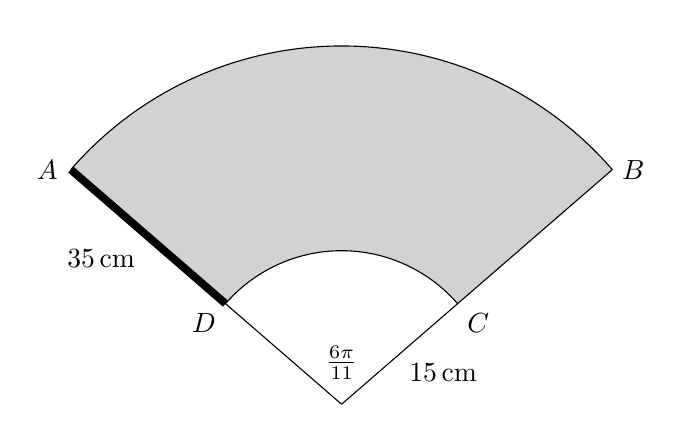
\begin{tikzpicture}[scale=1.3]
            
            \fill[gray!35] (0,0) -- (2.64512, 2.29201) -- (2.64512, 2.29201) arc [start angle=40.909, delta angle=98.182, radius=3.5cm] -- (-2.64512, 2.29201) -- (0,0) -- cycle;

            \fill[white] (0,0) -- (1.1336, 0.9823 ) -- (1.1336, 0.9823 ) arc [start angle=40.909, delta angle=98.182, radius=1.5cm] -- (-1.1336, 0.9823 ) -- (0,0) -- cycle;

            \draw[] (0,0) -- node[below right]{$15$\,cm}(1.1336, 0.9823 )
            node[below right]{$C$};
            \draw[] (0,0) -- (-1.1336, 0.9823 )
            node[below left]{$D$};

            \draw [] (1.1336, 0.9823 ) -- (2.64512, 2.29201) node[right]{$B$};
            \draw[line width=1mm] (-1.1336, 0.9823 ) -- node[below left]{$35$\,cm}(-2.64512, 2.29201) node[left]{$A$};

            \draw (1.1336, 0.9823) arc [start angle=40.909, delta angle=98.182, radius=1.5cm];
            \draw (2.64512, 2.29201) arc [start angle=40.909, delta angle=98.182, radius=3.5cm];

            \coordinate[label=above:$\frac{6\pi}{11}$] (O) at (0,0.15);
            
        \end{tikzpicture}
    \end{center}

    \begin{parts}
    \part[1] Find the length of the arc $AB$, correct to two decimal places.
    \fillwithdottedlines{25mm}
    \part[2] Find the area of the region $ABCD$, correct to two decimal place.
    \fillwithdottedlines{49mm}
    \end{parts}

\question[3] Prove that $\sec \gamma +\tan \gamma + \cot \gamma = \dfrac{1 + \sin \gamma}{\sin \gamma \cos \gamma}$
\fillwithdottedlines{49mm}

\question[2] Simplify $\dfrac{\cos ^{2} \theta}{1 + \sin \theta} + \dfrac{\cos ^{2} \theta}{1 - \sin \theta}$.
\fillwithdottedlines{41mm}

\question Solve for $x$, where $0 \le x < 2\pi$:
    \begin{parts}
    \part[2] $\cos x = - \dfrac{1}{\sqrt{2}}$
    \fillwithdottedlines{41mm}
    \part[3] $2 \cos ^{2} x = \sin x +1$
    \fillwithdottedlines{49mm}
    \part[3] $\sin x - \sqrt{3} \cos x = 0$
    \fillwithdottedlines{49mm}
    \end{parts}


\newpage

\question[4]
    Two surveyors, $A$ and $B$, stand on level ground to observe a large tree. Surveyor $A$ sights the top of the tree on an angle of elevation of $52^{\circ}$. 
    Surveyor $B$ sights the top of the tree on an angle of elevation of $46^{\circ}$.
    Surveyor $B$ is 27 metres away from Surveyor $A$ on a bearing of $47^{\circ}$. The tree is directly north of surveyor $A$.
    Find the height, $h$, of the tree correct to the nearest metre.
    \makeemptybox{75mm}
    \fillwithdottedlines{96mm}

\end{questions}
\nomorequestions

\vspace*{35mm}
\begin{center}
    \textbf{\textit{The End}}
\end{center}